\documentclass{article}
\usepackage[utf8]{inputenc}
\usepackage{makecell,tabularx} % <-- added tabularx
\usepackage{lipsum}% for dummy text
\usepackage{listings} %for making tables
\usepackage{amsmath} % for math equations
\usepackage{todonotes} %for todo notes


\title{Exploration and Presentation - Assignment 2 - Task 2}
\author{Martin Høigaard Rasmussen }
\date{March 2021}

\usepackage{natbib}
\usepackage{graphicx}

\begin{document}

\maketitle

\tableofcontents

\section{Danish characters}
æ ø å

\section{Graphics}

\subsection{Image with caption over it}
\todo{make images appear in correct places}
\begin{figure}[!ht]
  \centering
  \caption{A picture of the universe!}
  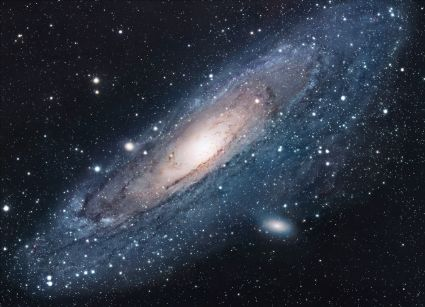
\includegraphics[width=0.5\textwidth]{universe}
\end{figure}

\subsection{Image with caption below it}

\begin{figure}[!ht]
  \centering
  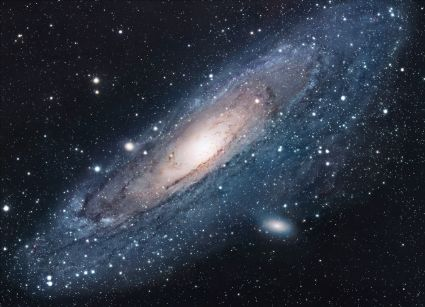
\includegraphics[width=0.5\textwidth]{universe}
    \caption{A picture of the universe!}
\end{figure}

\subsection{Image label}
\begin{figure}[!ht]
  \centering
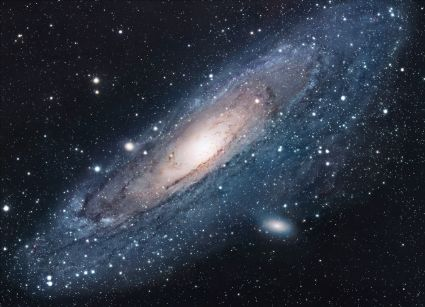
\includegraphics[]{universe.jpg}
\label{fig:spiralgalaxy}
\end{figure}

This is a label that references \ref{fig:spiralgalaxy} on page \pageref{fig:spiralgalaxy}

\subsection{Images next to each other}

\begin{figure}[!tbp]
  \centering
  \begin{minipage}[b]{0.4\textwidth}
    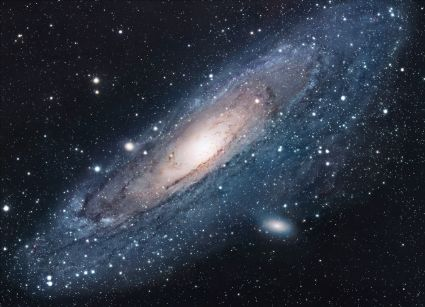
\includegraphics[width=\textwidth]{universe.jpg}
    \caption{image one.}
  \end{minipage}
  \hfill
  \begin{minipage}[b]{0.4\textwidth}
    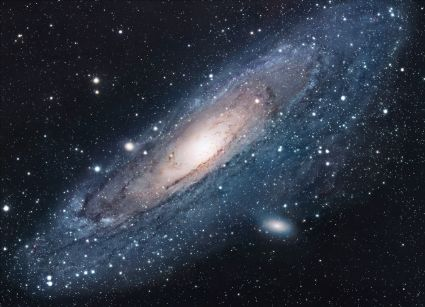
\includegraphics[width=\textwidth]{universe.jpg}
    \caption{image two.}
  \end{minipage}
\end{figure}

\section{Sections}
This is a section
    \subsection{Subsection}
    This is a subsection
    \subsubsection{Sub subsection}
    This is a sub subsection
    \subsection*{Unnumbered subsection}
    This is an unnumbered subsection
    
    
\section{Lists}
    \subsection{Bullet points}
        \begin{itemize}
            \item One entry in the list
            \item Another entry in the list
        \end{itemize}
    
    \subsection{Alternate bullet symbols}
        \begin{list}{$\circ$}{}
            \item One entry in the list with alternative symbol
            \item Another entry in the list with alternative symbol
        \end{list}
  
    \subsection{Enumerated lists}
        \begin{enumerate}
   \item First level item
   \item First level item
   \begin{enumerate}
     \item Second level item
     \item Second level item
     \begin{enumerate}
       \item Third level item
       \item Third level item
       \begin{enumerate}
         \item Fourth level item
         \item Fourth level item
       \end{enumerate}
     \end{enumerate}
   \end{enumerate}
 \end{enumerate}


    \subsubsection{Alternate enumerated list in Roman literals}
  \renewcommand{\theenumi}{\Roman{enumi}}%
\begin{enumerate}
  \item One
  \item Two
  \item Three
\end{enumerate}

\section{Table with multiple columns}
\subsection{Various horizontal alignments in columns (left, center, right)}

\begin{center}
\begin{tabular}[t]{ |l|c|r| } 
 \hline
 Left aligned & Center aligned & Right Aligned \\ 
 \hline
 cell1 & cell2 & cell3 \\ 
 \hline
 cell4 & cell5 & cell6 \\ 
 \hline
 cell7 & cell8 & cell9 \\ 
 \hline
\end{tabular}
\end{center}

\subsection{Cell spanning multiple Columns}


\begin{center}
\begin{tabular}{|c|c|}
    \hline
    \multicolumn{2}{|c|}{Multi-column}\\
        \hline
    Column 1 value & Column 2 value \\
    \hline
\end{tabular}
\end{center}


\subsection{Vertical alignment in multi-line cells}
    
\begin{center}

\begin{tabular}{|c|c|c|c|}
  \hline
\thead{a few rows\\ of text}
&   \thead{a few rows \\ of text}
&   \thead{a few rows\\ of text}
&   \thead{a few more\\ more rows\\ of text} \\
  \hline
Three & Four & 5 & 6 \\
  \hline
\end{tabular}
\end{center}

    
\subsection{Table description, label and reference}

\begin{table}[t]
\centering
\caption{This is a table caption/description}
\begin{tabular}{|l|c|c|c|c|c|}
\hline
Product & 1 & 2 & 3 & 4 & 5\\
\hline
Price & 124.- & 136.- & 85.- & 156.- & 23.-\\
Guarantee [years] & 1 & 2 & - & 3 & 1\\
Rating & 89\% & 84\% & 51\% & & 45\%\\
\hline
\hline
Recommended & yes & yes & no & no & no\\
\hline
\end{tabular}

\label{table:label}
\end{table}
This is a reference to table \ref{table:label}

\section{Code listing}

\subsection{Verbatim}
\begin{verbatim}
Text enclosed inside \texttt{verbatim} environment 
is printed directly 
and all \LaTeX{} commands are ignored.
\end{verbatim}

\subsection{With emphasized key words in your favorite programming language (python in example below)}

\begin{lstlisting}[language=Python]
import numpy as np
    
def incmatrix(genl1,genl2):
    m = len(genl1)
    n = len(genl2)
    M = None #to become the incidence matrix
    VT = np.zeros((n*m,1), int)  #dummy variable
    
    #compute the bitwise xor matrix
    M1 = bitxormatrix(genl1)
    M2 = np.triu(bitxormatrix(genl2),1) 

    for i in range(m-1):
        for j in range(i+1, m):
            [r,c] = np.where(M2 == M1[i,j])
            for k in range(len(r)):
                VT[(i)*n + r[k]] = 1;
                VT[(i)*n + c[k]] = 1;
                VT[(j)*n + r[k]] = 1;
                VT[(j)*n + c[k]] = 1;
                
                if M is None:
                    M = np.copy(VT)
                else:
                    M = np.concatenate((M, VT), 1)
                
                VT = np.zeros((n*m,1), int)
    
    return M
\end{lstlisting}

\section{Math equations}
\subsection{Inline - in text}
The well known Pythagorean theorem \(x^2 + y^2 = z^2\) was 
proved to be invalid for other exponents. To put your equations in inline mode use one of these delimiters:

\verb| \( \), $ $ or \begin{math} \end{math}|




\subsection{Display equations (on separate line)}
To put your equations in separate line mode use these delimiters:
\verb| \[ \] , $$ $$|
\[ x^n + y^n = z^n \]

\subsection{Fractions, summations, products, roots, powers}
\subsubsection{Fractions}
$$\tfrac{x}{y}$$

\subsubsection{Summations}

\[ \sum_{n=1}^{\infty} 2^{-n} = 1 \]

\subsubsection{Products}
\[ \prod_{i=a}^{b} f(i) \]

\subsubsection{Roots}
$$ \sqrt[n]{x} $$

\subsubsection{Powers}
$$ x^{n} $$

\section{Bibliography}
\todo{make links work in bibliography}
\nocite{*}
\bibliographystyle{plain}
\bibliography{references.bib}
\end{document}